% elemCell.tex      pdflatex ZhCvGo15
% Diffuse globally, compute locally: a cyclist tale
% Tingnan Zhang, Daniel I. Goldman and Predrag Cvitanovi\'c

%was \section{Cycles in the elementary cell}
%\label{s-elemCell}


The computation of diffusion coefficient \refeq{eq-diff-ec} requires
knowledge of \po s. In the Lorentz gas system, a few simple orbits may be
obtained by inspection: a 2-bounce \po\ is traced out by the particle
bouncing between a disk and one of its nearest neighbors, or one of the
second nearest disks. The number of \po s increases exponentially with
$\cl{p}$, the number of bounces (the `topological length' of the
orbit), they trace out shapes of increasing spatial complexity, and as
their instability increases exponentially with their length, it
becomes quickly not possible to determine them with the initial guess
Newton's method.

Instead, we need to first enumerate qualitatively all possible
trajectories, \ie, construct the \emph{symbolic dynamics} for the system.
The idea is to identify each \po\ with a unique sequence of symbols,
drawn from a finite alphabet. Intuitively speaking, a symbol may
characterize a certain pattern of the dynamics. Once the alphabet and the
grammar of admissible itineraries is determined, we may enumerate all
possible \po s and eventually pin down as many as needed for the
computation of a given long-time average.

We start with a brief review of the symbolic dynamics developed in
\refref{CGS92}. With imposed finite horizon there are 12 possible ways of
jump from a disk (\reffig{fig-diskDirectionsElCell}\,(a)). Any trajectory
in the full space can always be constructed from a series of flights,
each belongs to the 12 ``signature jumps''. In particular, a \po\ in the
elementary cell is represented as a repeatable string of such symbols.
For example, the bouncing mode between nearest disks is written as
\cycle{06}, meaning that the \po\ is consisted of two successive flights,
one traveling towards right (symbol $0$) and the
next reflecting backwards (symbol $6$).

Periodic orbits in the elementary cell can either be \emph{stationary} in
the full \statesp\ (returning to its initial point after completing a
full cycle, e.g., \cycle{06} that bounces between two nearest disks); or
\emph{running}, with a net spatial displacement after each period (e.g.,
\cycle{05}, \reffig{fig-diskDirectionsElCell}\,(a) and (c)). A stationary
cycle ``traps'' the  particle locally for all time, while a running cycle
advances it at a constant  velocity. The diffusion \refeq{eq-diff-ec} is
the result of competition between the two type of cycles.

With the symbolic dynamics, we then use the least action principle to
compute the \po s\rf{DasBuch}. In a planetary Hamiltonian
billiard system, the Maupertuis' principle indicates that the
traveling length along a cycle is minimized. We can solve the problem
by optimizing the total free flight distance with the constraint that
links have to connect the specific disks visited along the orbit.

\begin{figure}
  \begin{center}
    (a)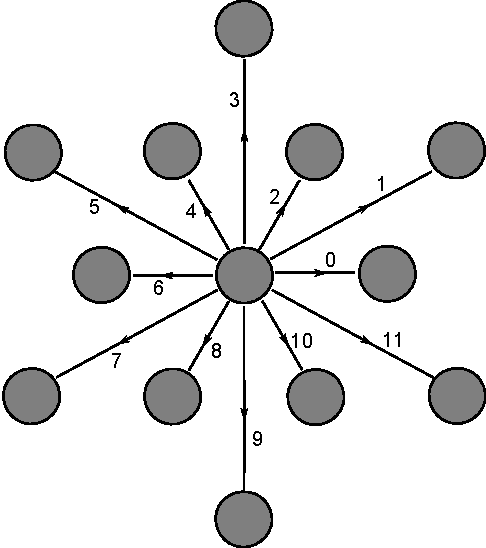
\includegraphics[width=0.27\textwidth]{diffuseDiskDirectionsElCell}
    (b)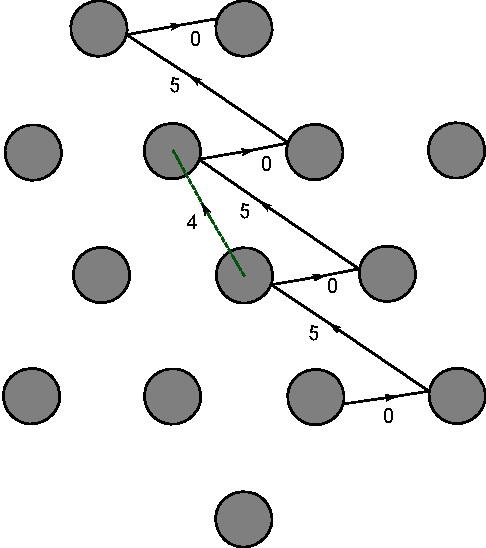
\includegraphics[width=0.27\textwidth]{diffuseDiskDirecsElCell05}
    (c)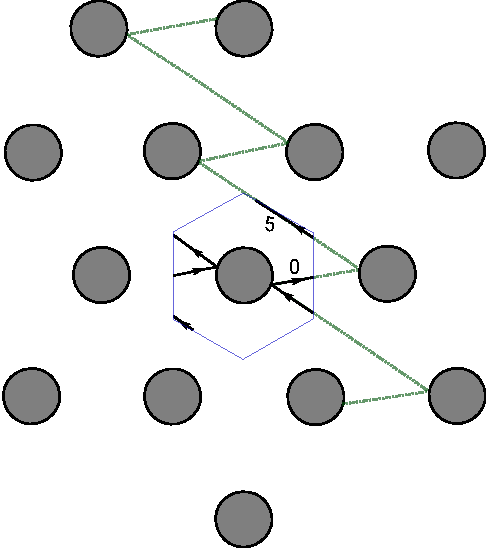
\includegraphics[width=0.27\textwidth]{diffuseDiskDirecsElCell05red}
  \end{center}
  \caption{\label{fig-diskDirectionsElCell}
  Elementary cell symbolic dynamics is obtained by counterclockwise
  labeling the translation vectors connecting the center of the current
  disk to the center of  the next disk. (a) The finite horizon is here
  imposed by limiting jumps from  the center cell to six short jumps
  (even labels $0, 2,\cdots,10$) and six `long' jumps (odd labels $1,
  3,\cdots,11$). (b) Running mode  \cycle{05} advances by $\hn_4$ per
  period. (c) In the elementary cell this is  a \po\ \cycle{05} of
  topological length 2.
  }
\end{figure}

Some confidence can be gained at this point by applying the above
formula~\refeq{eq-diff-ec} to a trivial system. For a simple example,
see the chain of baker's maps chain of coupled baker maps studied in
\refref{Gaspard92}.

In this case there are only four fixed points, all with stability
$\Lambda_p=1/2$, two of which give rise to the translations
$\hn_{p}=\pm 1$. As the system is uniformly hyperbolic, all curvature
terms are identically zero, and the fixed points substituted into
\refeq{eq-diff-ec} yield immediately the correct result $D=1/4$.
